\documentclass[10pt]{article}
%% Specify the Express journal you are submitting to
%\usepackage[OME]{express}
\usepackage[OE]{express}
%\usepackage[BOE]{express}

\begin{document}
\title{Simple template for authors submitting to OSA Express Journals}

\author{Author One,\authormark{1} Author Two,\authormark{2,*} and Author Three\authormark{2,3}}

\address{\authormark{1}Peer Review, Publications Department, The Optical Society, 2010 Massachusetts Avenue NW, Washington, DC 20036, USA\\
\authormark{2}Publications Department, The Optical Society, 2010 Massachusetts Avenue NW, Washington, DC 20036, USA\\
\authormark{3}Currently with the Department of Electronic Journals, The Optical Society, 2010 Massachusetts Avenue NW, Washington, DC 20036, USA}

\email{\authormark{*}opex@osa.org} %% email address is required

% \homepage{http:...} %% author's URL, if desired

%%%%%%%%%%%%%%%%%%% abstract and OCIS codes %%%%%%%%%%%%%%%%
%% [use \begin{abstract*}...\end{abstract*} if exempt from copyright]

\begin{abstract}
Updated 13 July 2016. A simple template with some examples is provided for preparing \textit{Optics Express}, \textit{Biomedical Optics Express}, and \textit{Optical Materials Express} manuscripts in \LaTeX. For complete instructions, please open the detailed template with formatting guidelines at \href{http://www.overleaf.com/docs?template=osa-opex-guide}{Overleaf}.
\end{abstract}

\ocis{(000.0000) General; (000.2700) General science.} % REPLACE WITH CORRECT OCIS CODES FOR YOUR ARTICLE, MINIMUM OF TWO; Avoid using the OCIS codes for “General” or “General science” whenever possible.
%For a complete list of OCIS codes, visit: https://www.osapublishing.org/oe/submit/ocis/

%%%%%%%%%%%%%%%%%%%%%%% References %%%%%%%%%%%%%%%%%%%%%%%%%
\begin{thebibliography}{99}

\bibitem{gallo99} K. Gallo and G. Assanto, ``All-optical diode based on second-harmonic generation in an asymmetric waveguide,'' \josab {\bfseries 16}(2), 267--269 (1999).

\end{thebibliography}

%%%%%%%%%%%%%%%%%%%%%%%%%%  body  %%%%%%%%%%%%%%%%%%%%%%%%%%
\section{Introduction}

Standard \LaTeX{} or AMS\TeX{} environments should be used to place tables, figures, and math. Examples are given below.

\begin{verbatim}
\begin{figure}[htbp]
%\centering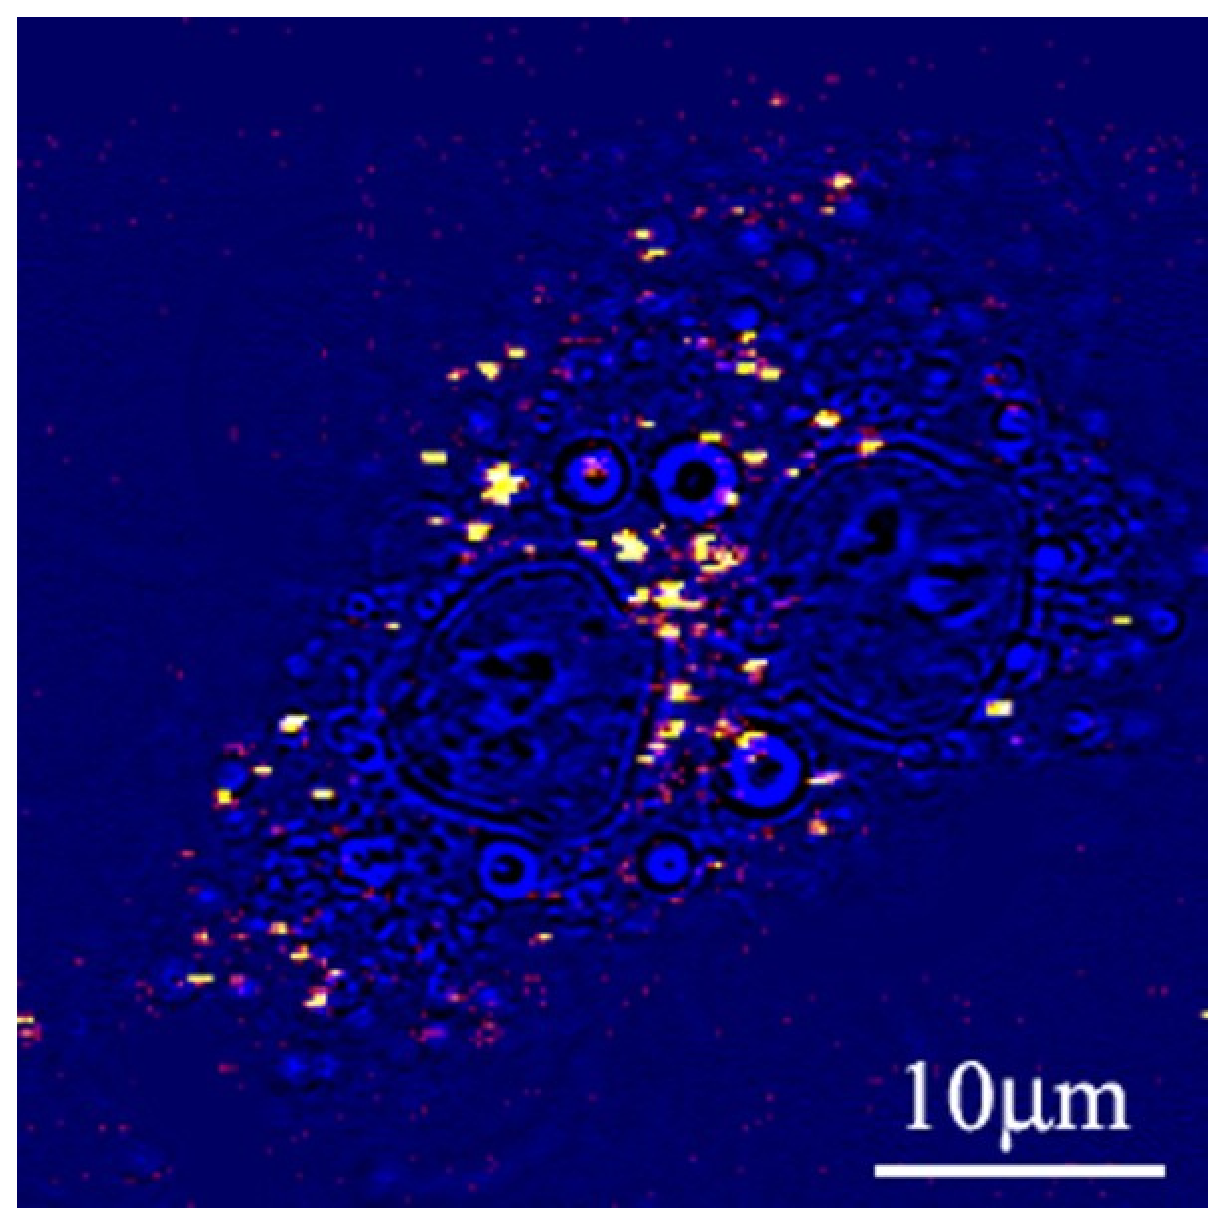
\includegraphics[width=7cm]{opexfig1}
\caption{Sample caption (Ref. \cite{Oron03}, Fig. 2).}
\end{figure}

\begin{equation}
H = \frac{1}{2m}(p_x^2 + p_y^2) + \frac{1}{2} M{\Omega}^2
     (x^2 + y^2) + \omega (x p_y - y p_x).
\end{equation}
\end{verbatim}

\section{Conclusion}
After proofreading the manuscript, compress your .TEX manuscript file and all figures (which should be in EPS format, or PDF format if you are using PDF-\LaTeX) in a ZIP, TAR or TAR-GZIP package. Prism, OSA’s article tracking system, will process in \LaTeX mode by default but will use PDF-\LaTeX if PDF figure files are detected. Note: TAR or TAR-GZIP is no longer required. All files must be referenced at the root level (e.g., file \texttt{figure-1.eps}, not \texttt{/myfigs/figure-1.eps}). If there is video or other multimedia, the associated files should be uploaded separately.

\section*{Funding}
Please identify all appropriate funding sources by name and contract number. Funding information should be listed in a separate block preceding any acknowledgments.

List only the funding agencies and any associated grants or project numbers, as shown in the example below:\\
National Science Foundation (NSF) (1253236, 0868895, 1222301); Program 973 (2014AA014402); Natural National Science Foundation (NSFC) (123456).

OSA participates in \href{http://www.crossref.org/fundingdata/}{Crossref's Funding Data}, a service that provides a standard way to report funding sources for published scholarly research. To ensure consistency, please enter any funding agencies and contract numbers from the Funding section in Prism during submission or revisions.


\section*{Acknowledgments}
Acknowledgments, if included, should appear at the end of the document. The section title should not follow the numbering scheme of the paper. Use the command \verb+\section*{Acknowledgments}+  to create a nonnumbered section heading. 

\end{document}
